\providecommand\ExamFontPath{../../../字体/}
\documentclass[fontset=exam]{exam-zh}
\usepackage{longtable,booktabs,array,calc,multirow,fvextra}
\usepackage[normalem]{ulem}
\providecommand{\hl}[1]{#1}
\providecommand{\ul}[1]{\uline{#1}}
\DefineVerbatimEnvironment{verbatim}{Verbatim}{breaklines=true,fontsize=\small}
\providecommand{\tightlist}{\setlength{\itemsep}{0pt}\setlength{\parskip}{0pt}}
\newcommand{\pandocbounded}[1]{#1}
\setlength{\emergencystretch}{3em}
\setlength{\tabcolsep}{2pt}
\examsetup{page/size=a4paper}
\title{厦门大学 期末考试}
\subject[4em]{热学}
\begin{document}
\maketitle
\fancyfoot[C]{第 \thepage 页（共 \pageref*{LastPage} 页）}
3.（15 分）

1mol 理想气体分别经以下两个准静态过程从 300K 加热至 350K：

（1）体积保持不变

（2）压强保持不变

设气体的定容摩尔热容\(C_{V,m} = \frac{3}{2}R\)，问这两个过程中各吸收多少热量？增加多少内能？对外做多少功？

4、（15 分）\par\medskip{\centering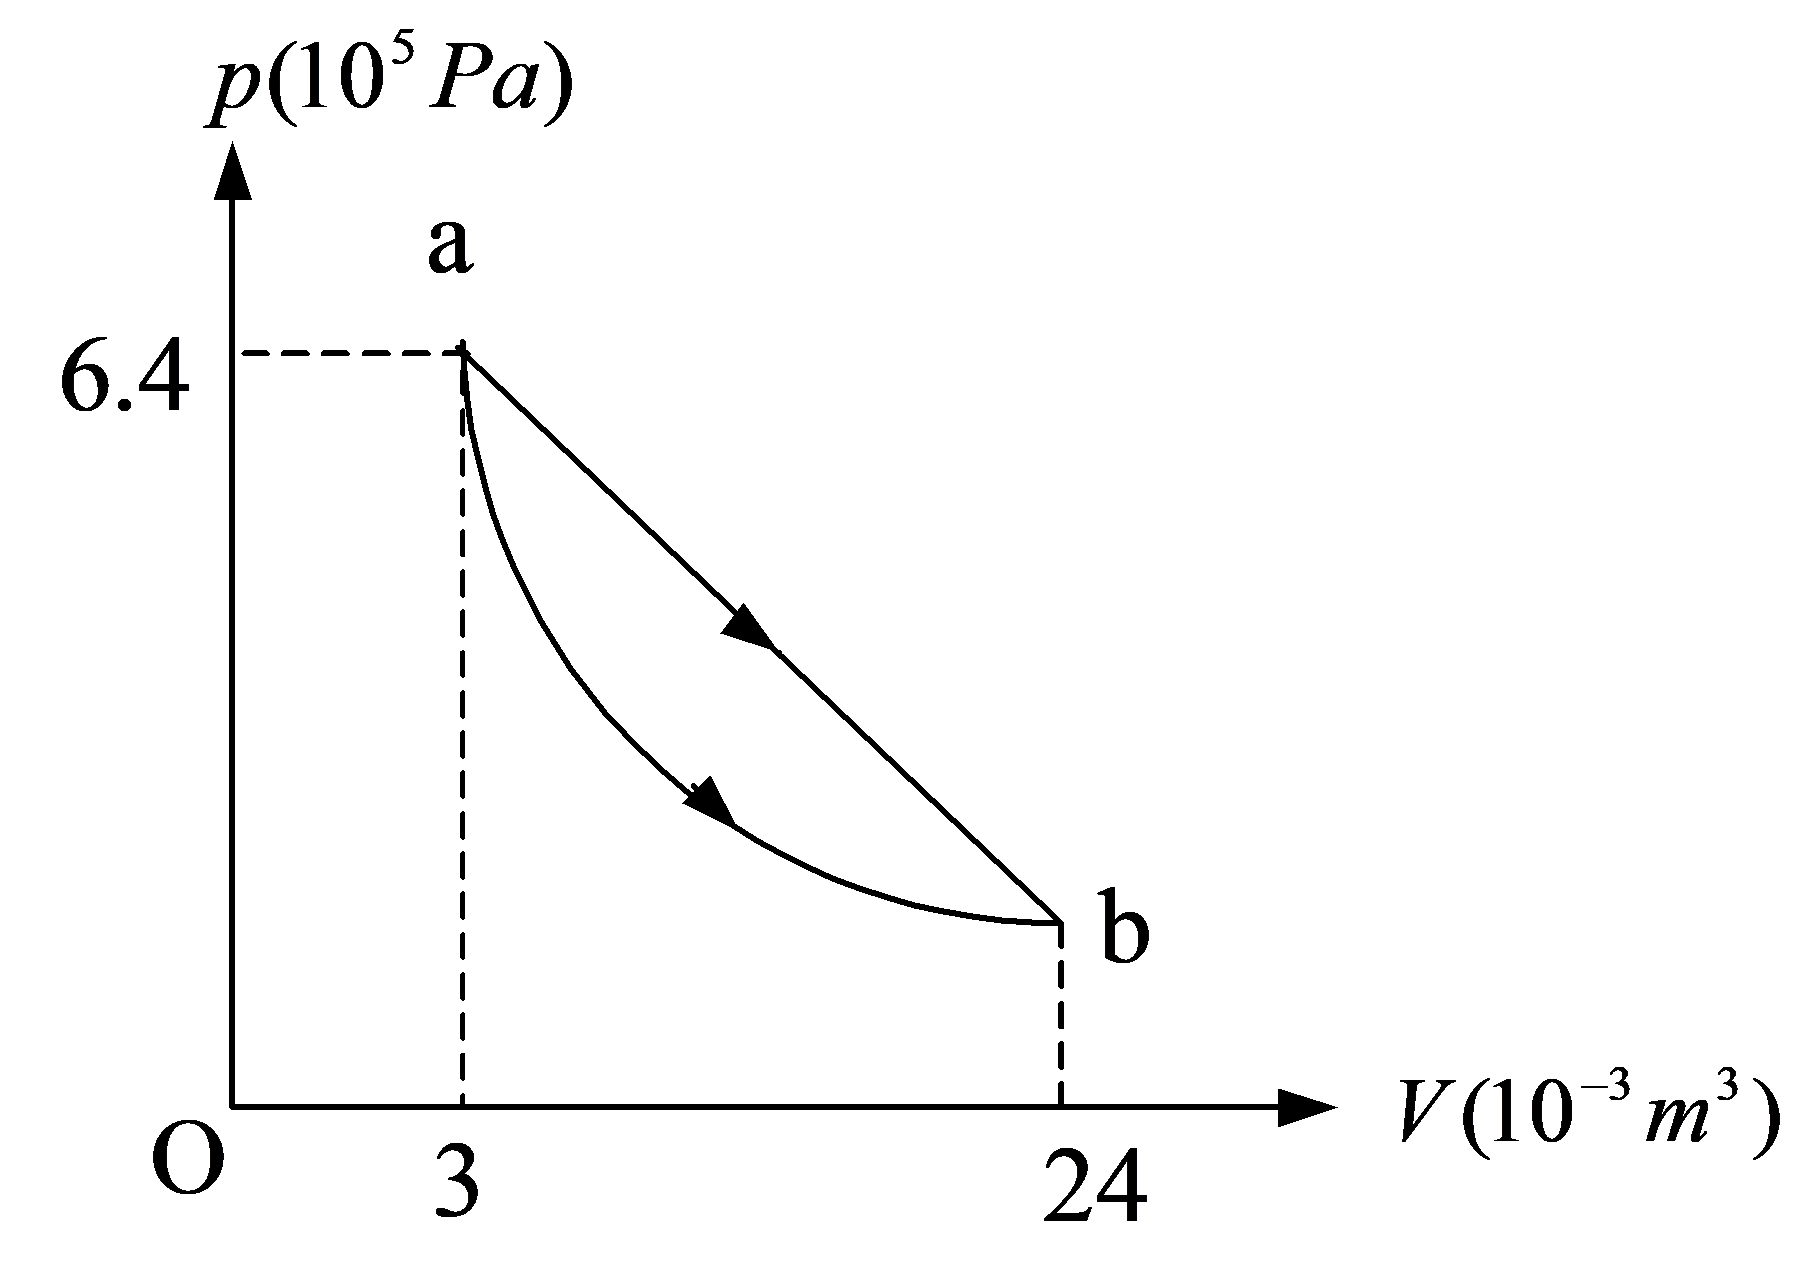
\includegraphics[width=5cm,height=4cm,keepaspectratio]{figures/image8.png}\par}\medskip

如图，某理想气体经一准静态绝热过程从状态 a 过渡到状态 b。设气体的定容摩尔热容\(C_{V,m} = \frac{3}{2}R\)，求系统对外所做的功。如系统经直线过程从 a 过渡到 b，则系统对外做功为多少？与外界之间交换的热量为多少？

5.（15 分）

1mol 理想气体经一准静态过程：\(V = \alpha\,\sqrt{T}\)（\(\alpha\)为常量）。已知该气体的定容摩尔热容量为\(C_{V,m} = \frac{5}{2}R\)（\emph{R}为气体普适为常量），求：

（1）系统温度从\(T_{1}\)变到\(T_{2}\)时气体所做的功\emph{A}；

（2）该过程的摩尔热容\emph{C}。

6．（15 分）\par\medskip{\centering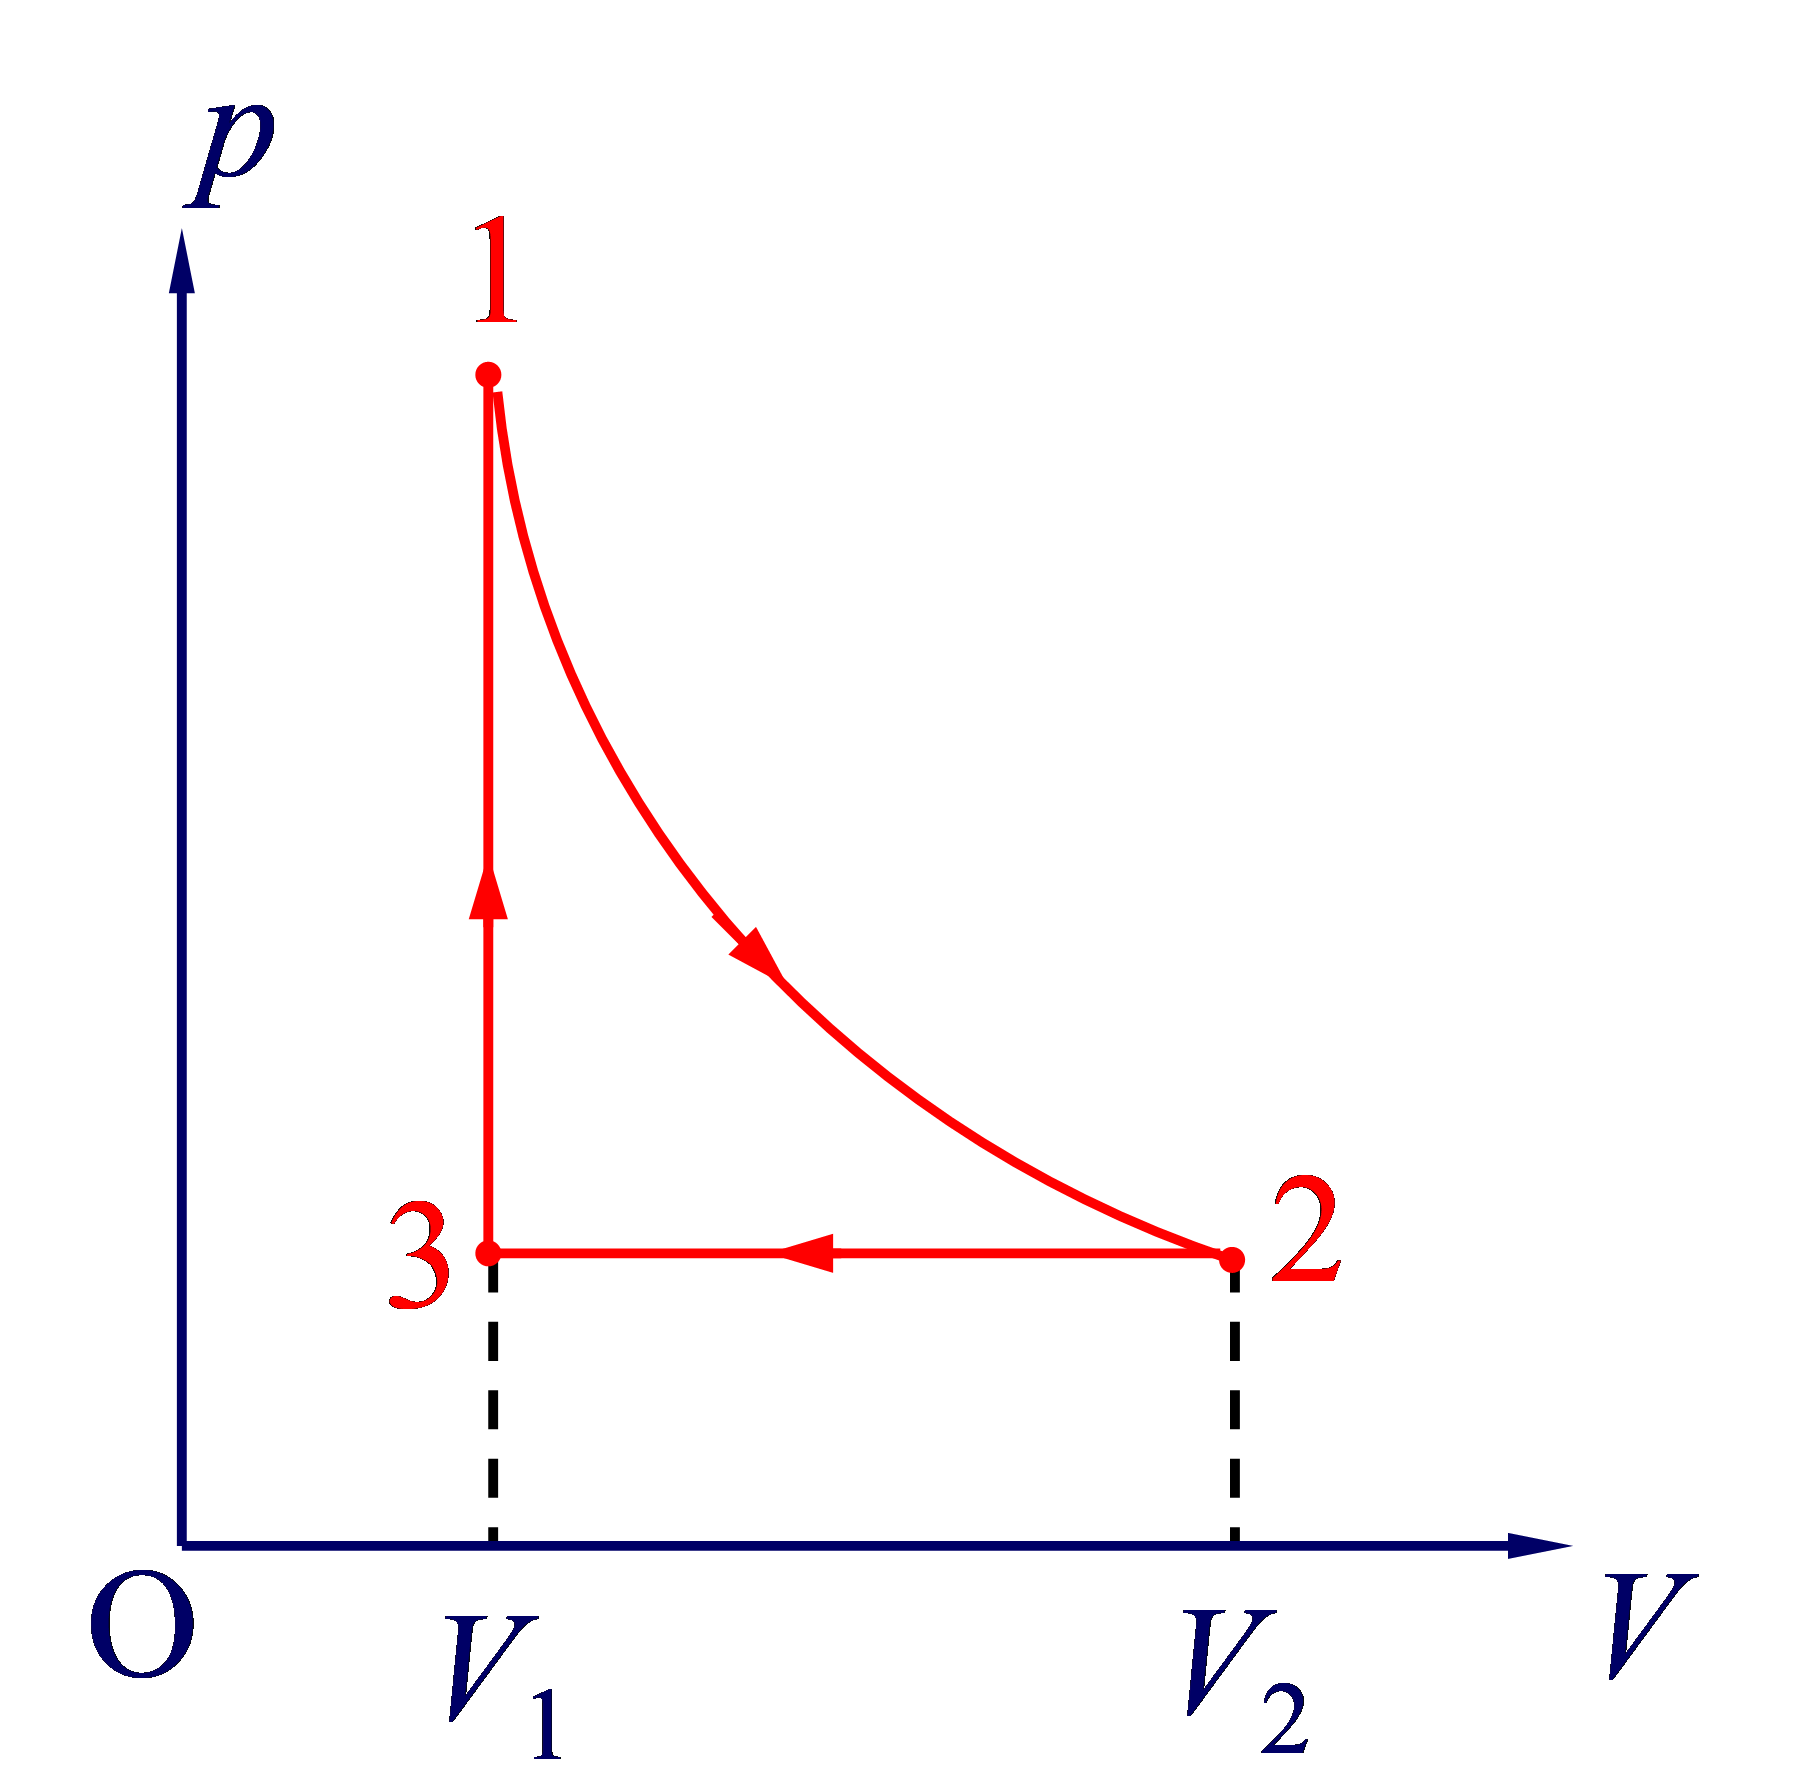
\includegraphics[width=5cm,height=4cm,keepaspectratio]{figures/image27.png}\par}\medskip

一热机的循环过程如图所示，其中 1\(\to\)2 为绝热过程，2\(\to\)3 为等压过程，3\(\to\)1 为等容过程。如工作物质为理想气体，其定容摩尔热容\(C_{V,m} = \frac{3}{2}R\)，\(V_{2} = 8V_{1}\)。

（1）求该热机的效率；

（2）若某一致冷机的循环过程为以上热机循环的逆循环，求该致冷机的致冷系数。

7．（10 分）

用一运转于\(T_{1} = 600K\)和\(T_{2} = 300K\)的高、低温热源之间的可逆热机推动一工作于\({T'}_{1} = 300K\)的热源和\({T'}_{2} = 250K\)的冷库之间的可逆冷机。为使制冷机每秒从冷库带走\(3.00 \times 10^{4}(J)\)的热量，热机每秒必须从高温热源吸收多少热量？

6.（10 分）

有一肥皂泡，当外界压强为\(p_{1}\)时，其半径为\(R_{1}\)，当外界压强为\(p_{2}\)时，其半径变为\(R_{2}\)，求肥皂泡的表面张力系数。（设肥皂泡内气体温度保持不变）。

7.（15 分）

一体积为\(20.0\)升的绝热密闭容器中储存有\(100^{0}\text{C}\)的饱和水蒸汽。现向其中注入少量温度为\(20^{0}\text{C}\)的液态水，达到平衡态时，水温变为\(80^{0}\text{C}\)。设水蒸汽的定容比热容为\(c_{1} = 1.38 \times 10^{3}\text{J} \cdot \text{k}\text{g}^{- 1} \cdot \text{K}^{- 1}\)，液态水的比热容为\(c_{2}{{}_{=}^{}4}.18 \times 10^{3}\text{J} \cdot \text{k}\text{g}^{- 1} \cdot \text{K}^{- 1}\)，水的汽化热\(l = 2.26 \times 10^{6}\text{J} \cdot \text{k}\text{g}^{- 1}\)，\(100^{0}\text{C}\)时水的饱和蒸汽压为\(p_{1} = 9.81 \times 10^{4}\text{P}\text{a}\)，\(80^{0}\text{C}\)时水的饱和蒸汽压为\(p_{2} = 4.81 \times 10^{4}\text{P}\text{a}\)，液态水所占的体积与容器体积相比可忽略不计。试求

（1）达到平衡态时，有多少质量的水蒸汽凝结成液态水？

（2）注入的液态水的质量是多少？

8.（10 分）

\begin{quote}
某物质摩尔汽化热\(L\)与温度的关系为\(L = L_{0} + RT\)，其中\(L_{0}\)为常数，\(R\)为气体普适常量。气液两相共存时，饱和蒸汽可近似为理想气体，且\(T = T_{0}\)时，饱和蒸汽压为\(p_{0}\)。试推导饱和蒸汽压与温度的关系。
\end{quote}

2. （18 分）

一定量的理想气体，初态体积为\emph{V}\textsubscript{0}，压强为\emph{p}\textsubscript{0}。先对气体等压加热，使体积膨胀为 2\emph{V}\textsubscript{0}，然后等容加热，使压强增大为 2\emph{p}\textsubscript{0} ，最后通过绝热过程使体积膨胀到 16 \emph{V}\textsubscript{0}。已知气体的定压摩尔热容\(C_{p,m} = \frac{5}{2}R\)（\emph{R}为气体普适常量），求

（1）全过程中内能的变化；

（2）全过程中气体吸收的热量和对外所做的功。

3. （18 分）

一根长为 76cm 的玻璃管，上端封闭，下端插入水银中，水银充满管子的一部分，管子另一部分封闭有 0.1mol 的空气，设外界压强保持在 76cmHg，空气的定容摩尔取\(C_{V} = \frac{5}{2}R\)。若管内空气的温度降低 10\textsuperscript{0}C，求：\par\medskip{\centering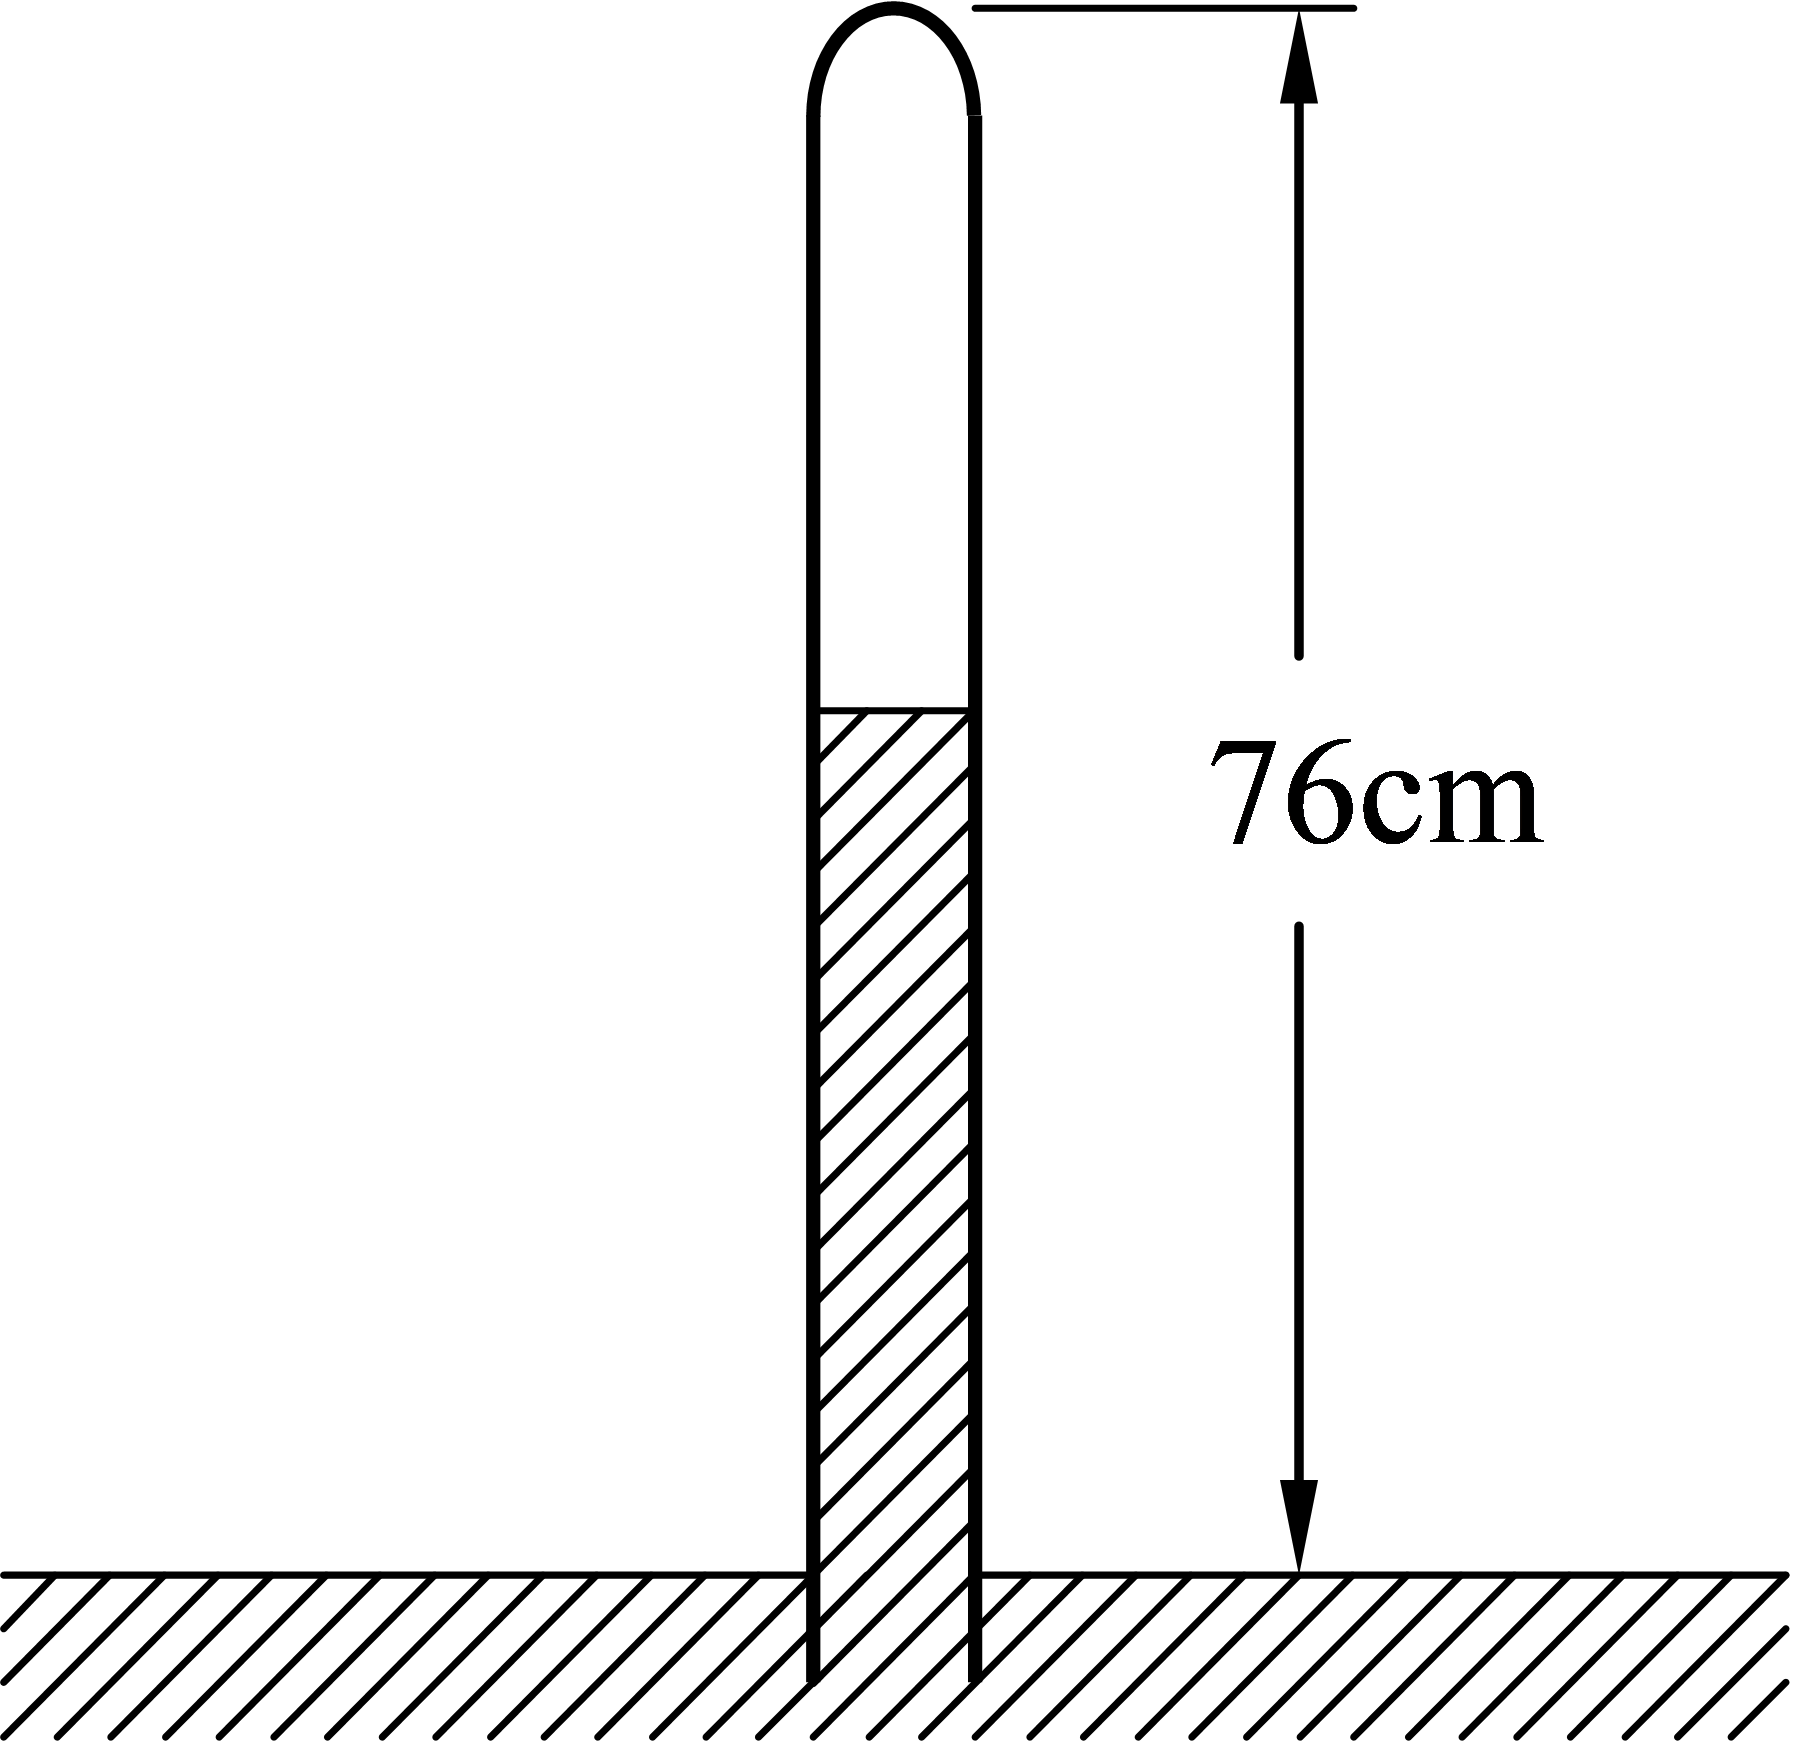
\includegraphics[width=5cm,height=4cm,keepaspectratio]{figures/image104.png}\par}\medskip

（1）管内空气内能的改变，是增大还是减小？

（2）管内空气对外所做的功，是正功还是负功？

（3）管内空气与外界交换的热量，是吸热还是放热？

4.（16 分）\par\medskip{\centering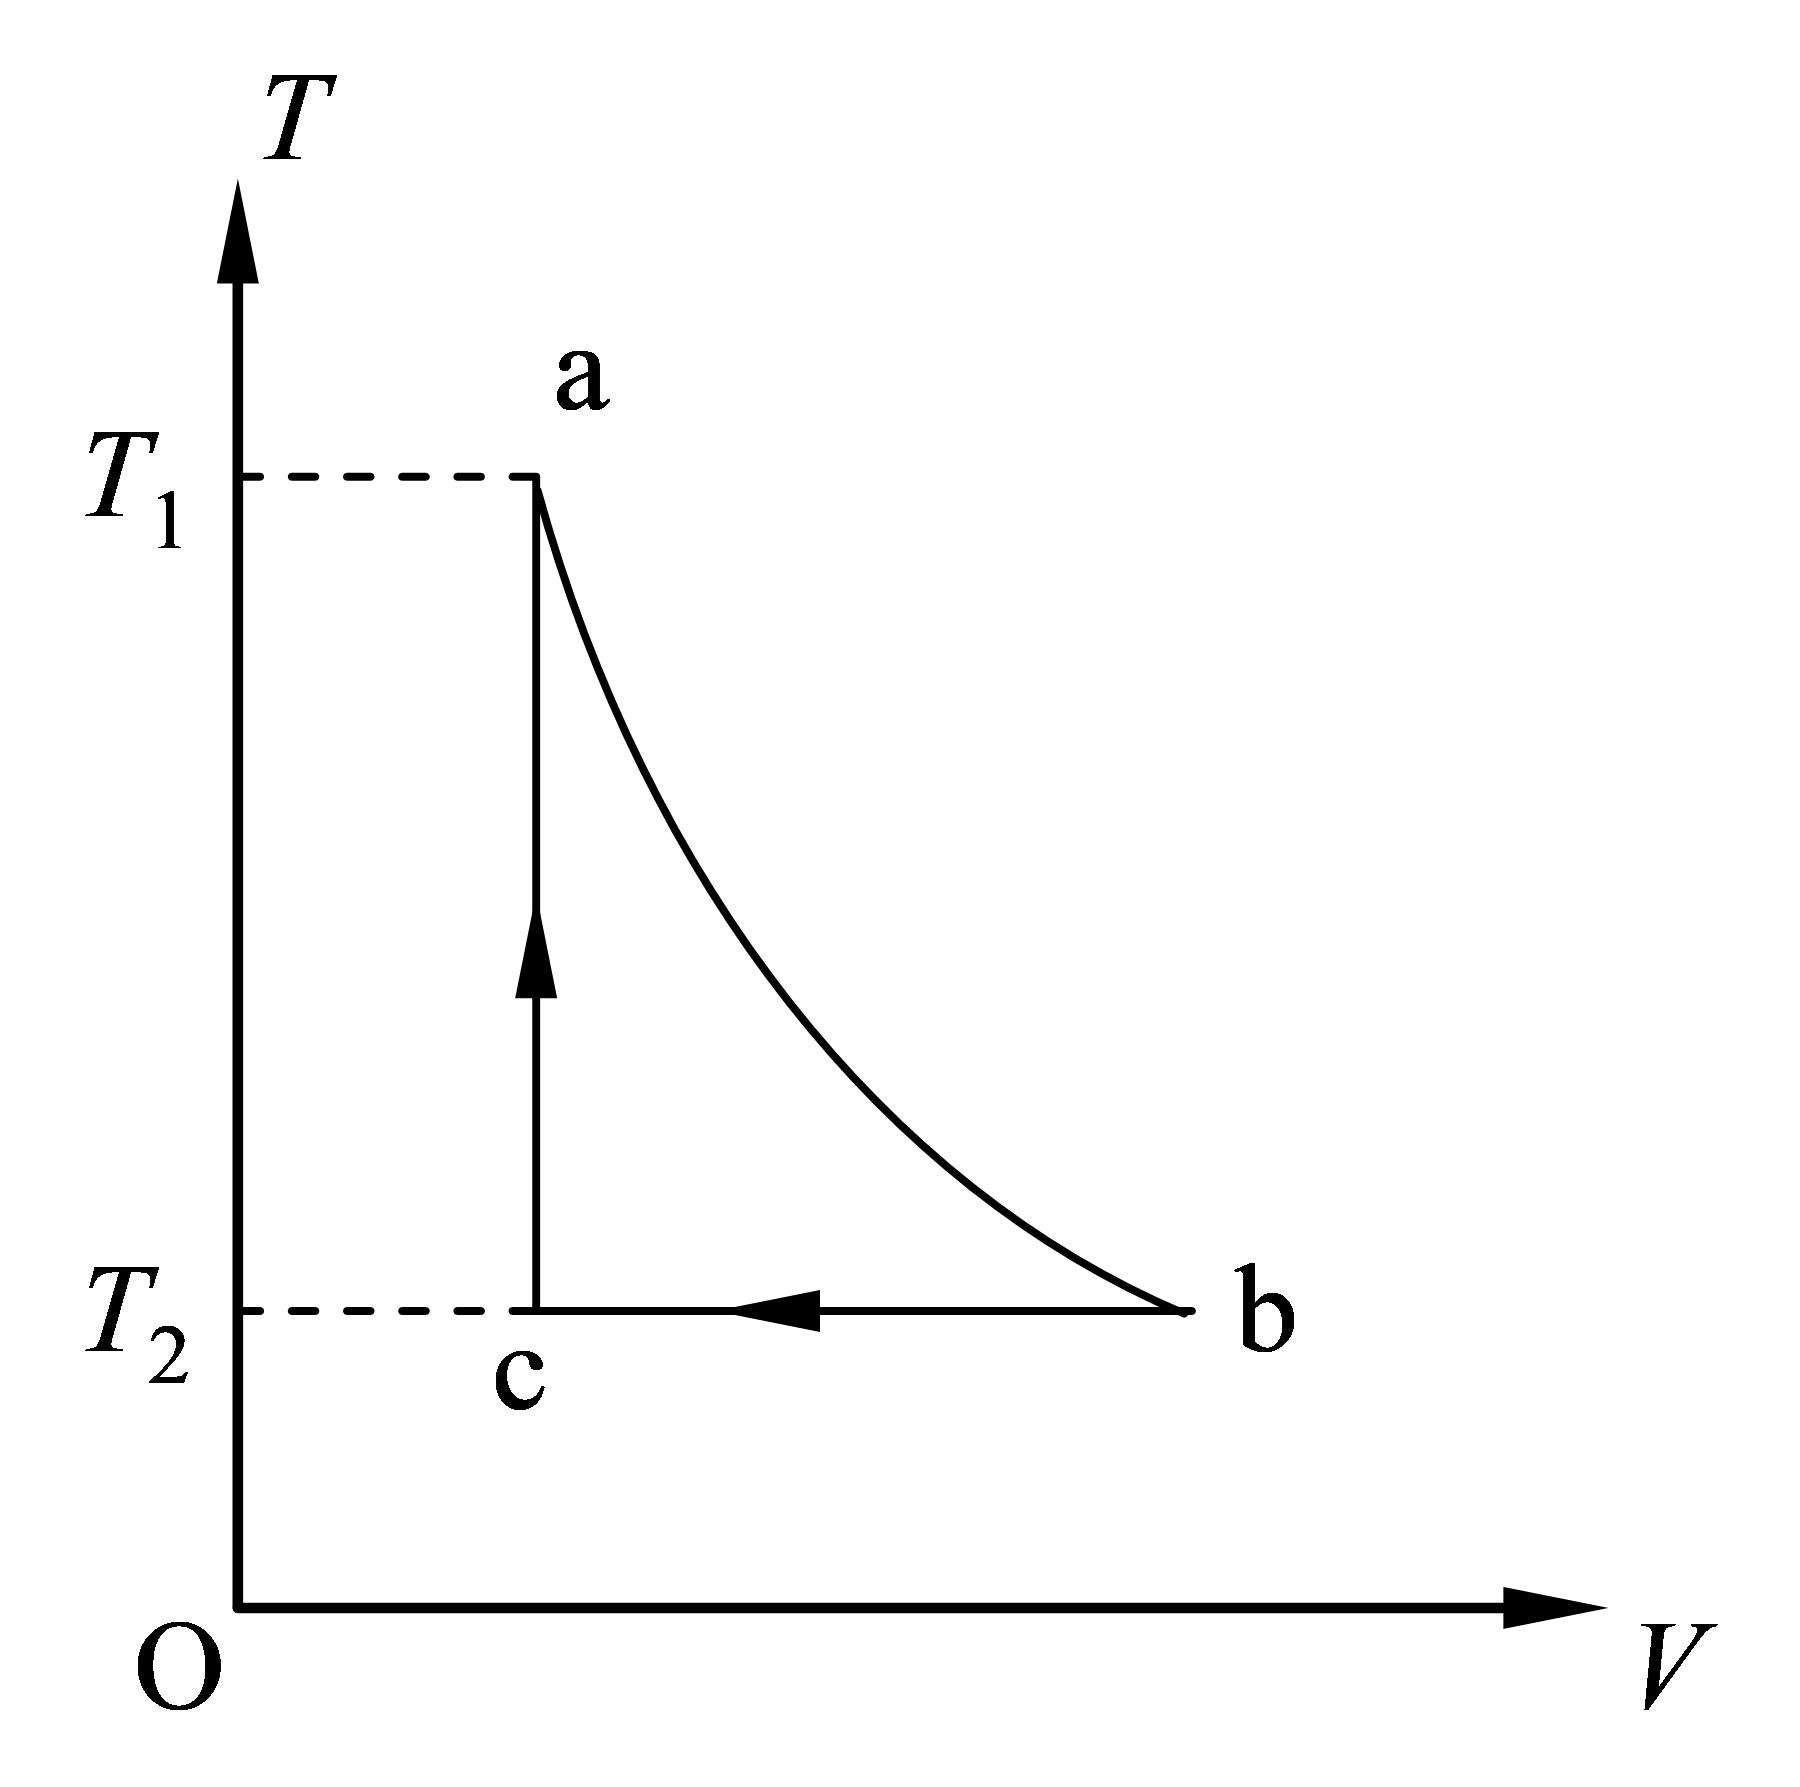
\includegraphics[width=5cm,height=4cm,keepaspectratio]{figures/image110.png}\par}\medskip

某热机的循环过程如图所示，其中 ab 为绝热过程，bc 为等温过程，ca 为等容过程。设工作物质为理想气体，证明热机的效率为

\[\eta = 1 - \frac{ln\beta}{\beta - 1}\]

式中\(\beta = T_{1}/T_{2}\)。

5．（15 分）

在温度分别为 227°C 和 27°C 的恒温热源之间工作的热机，在一个循环中从高温热源吸收的热量为 300J。

（1）假设该热机在一个循环中对外所做净功为 100J，则此热机是否为可逆热机，为什么？

（2）假设该热机为可逆热机，则在一个循环中对外所做净功为多少？

（3）假设该热机为可逆热机，今使其逆向运转，则为使在一个循环中工作物质从低温热源吸收 60J 的热量，外界对系统所做的净功是多少？

6.（15 分）

1mol 的理想气体分别经以下三个准静态过程使体积膨胀为原来的两倍：

（1）等压过程

（2）等温过程

（3）绝热过程

试分别求出上述三个过程中气体的熵变。设气体的定容摩尔热容\(C_{V,m} = \frac{3}{2}R\)（\emph{R}为气体普适常量）。

\end{document}
